%%%%%%%%%%%%%%%%%%%%%%%%%%%%%%%%%%%%%%%%%%%%%%%%%%%%%%%%%%%%%%%%%%%%%%%
%%%%%%%%%%%%%%%%%%%%%%%%%%%%%%%%%%%%%%%%%%%%%%%%%%%%%%%%%%%%%%%%%%%%%%%
%%%%%                                                                 %
%%%%%     <file_name>.tex                                             %
%%%%%                                                                 %
%%%%% Author:      <author>                                           %
%%%%% Created:     <date>                                             %
%%%%% Description: <description>                                      %
%%%%%                                                                 %
%%%%%%%%%%%%%%%%%%%%%%%%%%%%%%%%%%%%%%%%%%%%%%%%%%%%%%%%%%%%%%%%%%%%%%%
%%%%%%%%%%%%%%%%%%%%%%%%%%%%%%%%%%%%%%%%%%%%%%%%%%%%%%%%%%%%%%%%%%%%%%%


\chapter{Design Implementation and Results}
This chapter is about the architecture variant you actually
implemented and its resulting performance; e.g., SNR, image quality,
peak throughput, required bandwidth ... (whatever quality and
performance metrics apply). In an ASIC or FPGA project you would also
specify the key figures of your design; e.g., area/lut usage, timing
figures, interface widths... In an ASIC project you would also talk
about backend specific things such as the floorplan of your chip,
design for test (and test coverage), power simulation, special
clocking circuitry and pad/bonding diagrams.

\section{First Section}


\section{Second Section}

\section{Verification}

\subsection{Functional}
Do not forget to include information about how you managed to do the
functional verification (golden model, testbench,
etc.). Figure~\ref{fig:func_ver} illustrates an example setup.

\begin{figure}[tb]
  \centering
  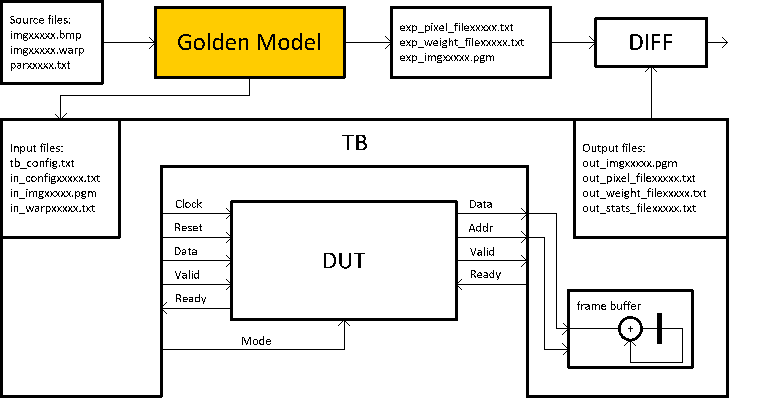
\includegraphics[width=\linewidth]{./figures/tb}
  \caption{Functional verification setup.}
  \label{fig:func_ver}
\end{figure}

\subsection{Design for Testability (DFT)}
\subsubsection{Automated Testpattern Generation}

\section{Results}
If you only have very few results, it might be a better approach to
insert them into this chapter (instead of putting the results into a
separate one).
